\chapter{Algorithmen}
\lhead{Algorithmen}
Nicht jeder Algorithmus ist f"ur High Performance Computing geeignet.
Nur wenn gen"ugend viele Rechenschritte soweit unabh"angig sind, dass sie
parallel auf vielen CPUs ausgef"uhrt werden k"onnen, besteht die
Chance, durch Parallelisierung die Leistung einer massiv parallelen Maschine
ausnutzen zu k"onnen. Dieses Kapitel zeigt einige Beispiel von ungeeigneten
Algorithmen und ihren HPC-tauglichen Gegenst"ucken.

F"ur die Eigenwerte und Eigenvektoren einer $n\times n$-Matrix $A$ 
lernt man in der linearen Algebra den folgenden Algorithmus:
\begin{enumerate}
\item Bestimme das charakteristische Polynom
$\chi_{A}(\lambda)=\det(A-\lambda I)$.
\item Finde die Nullstellen $\lambda_1,\lambda_2,\dots,\lambda_n$ von
$\chi_A(\lambda)$.
\item F"ur jede Nullstelle $\lambda_i$, finde eine nichttriviale L"osung $v_i$
des Gleichungssystems $(A-\lambda_i I)v_i=0$.
\end{enumerate}
Dieser Algorithmus funktioniert sehr gut bei kleinen Matrizen, aber sobald
$n$ gr"osser wird, ist der Algorithmus undurchf"uhrbar.
Nur schon die Berechnung des charakteristischen Polynoms mit Hilfe
der Determinante ist unm"oglich.
Aber auch die Berechnung der Eigenwerte als Nullstellen ist, abgesehen
von den numerischen Problemen dieses Unterfangens, in keiner Weise
parallelisierbar.

Das Eigenwertproblem ist nur eines von vielen praktisch wichtigen
Problemen, f"ur welches die Methoden, die man meist als erste lernt,
nicht geeignet sind. Auch die L"osung eines linearen Gleichungssystems
mit dem Gauss-Algorithmus wird unpraktikabel, wenn das Gleichungssystem
sehr gross ist, und wie in Anwendungsproblemen h"aufig der Fall ist,
nur wenige Matrix-Eintr"age von 0 verschieden sind.
Das Ziel dieses Kapitels ist daher, eine Reihe von Algorithmen dazustellen,
welche auch f"ur sehr grosse Probleme der linearen Algebra immer noch
effizient durchf"uhrbar sind.

\section{Iterative Methoden zur L"osung linearer Gleichungssysteme}
\rhead{Iterative Methoden}
In diesem Abschnitt suchen wir Methoden zur L"osung eines linearen
Gleichungssystems $Ax=b$ mit einer $n\times n$-Matrix $A$ und einem
$n$-dimensionalen Vektor $b$.
Die in der Praxis tats"achlich zu l"osenden Gleichungssysteme sind meist 
nicht beliebig, es ist daher auch nicht notwendig, L"osungen f"ur beliebige
Matrizen $A$ zu entwickeln.
In Abschnitt~\ref{section-motivation} betrachten wir daher an einem Beispiel,
wie in den Anwendungen lineare Gleichugnssysteme auftauchen, und versuchen,
die Charakteristiken dieser Gleichungssysteme herauszustellen. Die
nachfolgenden Abschnitte k"ummern sich dann nur noch um Methoden, die
f"ur diese Art von Gleichungsssystemen besonders gut geeignet sind.

\subsection{Motivation\label{section-motivation}}
Partielle Differentialgleichungen sind wichtige Lieferanten von 
linearen Gleichungssystemen in den Anwendungen.
Die Wetterentwicklung, elastische Deformation, Schwingung von
Maschinenteilen oder Geb"auden oder Ausbreitung von Wellen sind
Ph"anomene, die mit partiellen Differentialgleichungen beschrieben
werden k"onnen. In diesem Abschnitt wollen wir zeigen, wie eine
partielle Differentialgleichung zu einem linearen Gleichungssystem
Anlass gibt, und welche Eigenschaften dieses Gleichungssystem hat.

Als Beispiel betrachten wir die partielle Differentialgleichung
\begin{equation}
\Delta u
=\frac{\partial^2u}{\partial x^2}+\frac{\partial^2u}{\partial y^2}
=f(x,y),
\label{motivation-pdgl}
\end{equation}
welche das Potential (elektrisches Potential oder das Potential eines
Gravitationsfeldes) einer Ladungs- oder Massenverteilung mit
Dichte $f(x,y)$ beschreibt.
Gesucht ist eine Funktion $u(x,y)$, welche auf dem Einheitsquadrat
$\Omega = \{(x,y)\,|\, 0\le x,y\le 1\}$ definiert ist und auf dem Rand bestimmte
vorgegebene Werte annimmt:
\begin{equation}
u(x,y)=g(x,y)\qquad x\in\partial \Omega,
\label{motivation-randbedingung}
\end{equation}
wobei $\partial\Omega$ der Rand des Gebietes $\Omega$ ist. Die allgemeine
Theorie der partiellen Differentialgleichungen beweist, dass dieses
Problem eine eindeutige L"osung hat.
Im konkreten Fall eines rechteckingen Gebietes liefert die Theorie sogar
ein L"osungsverfahren, welches mindestens f"ur nicht zu komplizierte
Funktion $f$ und $g$ von Hand durchgef"uhrt werden kann.
F"ur beliebig geformte Gebiete $\Omega$ gibt es jedoch kein analytisches
L"osungsverfahren.

F"ur die numerische L"osung ersetzen wir die auf dem ganzen Quadrat
definierte Funktion $u(x,y)$ durch Zahlenwerte $u_{ij}$, welche nur
auf einem Gitter mit Knoten $(ih, jh)$ mit einer Gitterkonstanten $h = 1/n$
definiert sind.
Die Randbedingungen (\ref{motivation-randbedingung}) f"uhren unmittelbar
auf die Gleichungen
\begin{equation}
u_{ij}=g_{ij}=\begin{cases}
g(0,hj)&\qquad i = 0\\
g(1,hj)&\qquad i = n\\
g(hi,0)&\qquad j = 0\\
g(hi,1)&\qquad j = n
\end{cases}
\label{motivation-randwerte}
\end{equation}
Um die Differentialgleichung (\ref{motivation-pdgl}) durch lineare Gleichungen
zu ersetzen, muss eine Approximation der zweiten Ableitungen
gefunden werden.
Die erste Ableitung in $x$-Richtung kann angen"ahert werden durch
\begin{align*}
\frac{\partial u}{\partial x}(ih,jh)&\simeq \frac{u_{i+1,j}-u_{ij}}h
&
\frac{\partial u}{\partial y}(ih,jh)&\simeq \frac{u_{i,j+1}-u_{ij}}h.
\end{align*}
Daraus kann dann auch eine Approximation von der zweiten Ableitung
gefunden werden (siehe auch Abbildung~\ref{algorithm:laplacian}):
\begin{align*}
\frac{\partial^2 u}{\partial x^2}(ih,jh)&=\frac1h\biggl(
\frac{u_{i+1,j}-u_{ij}}h-\frac{u_{ij}-u_{i-j,j}}h
\biggr)
=\frac1{h^2}(u_{i-1,j}-2u_{ij}+u_{i+1,j}),\\
\frac{\partial^2 u}{\partial y^2}(ih,jh)&=
=\frac1{h^2}(u_{i,j-1}-2u_{ij}+u_{i,j+1}).
\end{align*}
\begin{figure}
\begin{center}
\includegraphics[width=0.7\hsize]{graphics/laplacian-1.pdf}
\end{center}
\caption{Diskretisation des Laplace-Operators an der Stelle $(x,y)=(ih, jh)$.
\label{algorithm:laplacian}}
\end{figure}
Die Differentialgleichung wir damit zu einer approximativen linearen
Gleichung 
\begin{equation}
\frac1{h^2}(u_{i-1,j}+u_{i,j-1}+u_{i+1,j}+u_{i,j+1}-4u_{ij})=f_{ij}=f(ih,jh)
\qquad 0<i,j<n.
\label{motivation-lingl}
\end{equation}
Statt der Differentialgleichung (\ref{motivation-pdgl}) mit den Randbedingungen
(\ref{motivation-randbedingung}) ist jetzt also das lineare Gleichungssystem
f"ur die $u_{ij}$ bestehend aus den Gleichungen (\ref{motivation-lingl}) und
(\ref{motivation-randwerte}) zu l"osen.
Die Randwertgleichungen legen einen Teil der $u_{ij}$ bereits fest,
man kann sie zur rechten Seite der Gleichungen schlagen,
so dass nur noch die Werte $u_{ij}$ an inneren Knotenstellen $0<i,j<n$
zu bestimmen.

Wir numerieren wir die verbleibenden Unbekannten neu mit einem
einzigen Index und nennen sie $U_k$,
\begin{equation}
\left.
\begin{aligned}
u_{ij}&=U_{j + (i - 1)(n - 1)}
\\
f_{ij}&=f_{j + (i-1)(n-1)}
\end{aligned}
\right\}
\quad 0<i,j<n.
\end{equation}
Die Gleichungen (\ref{motivation-lingl}) werden jetzt zu Gleichungen
f"ur die $U_k$:
\begin{equation}
U_{k-1}+U_{k+1}+U_{k-(n-1)}+U_{k+(n-1)}-4U_k=f_k.
\end{equation}
Die $(n-1)^2\times(n-1)^2$-Koeffizientenmatrix dieses Gleichungssystems ist
\[
A=\left(
\begin{array}{ccccc|ccccc|c|ccccc}
    -4&     1&     0&\cdots&     0 &     1&     0&     0&\cdots&     0 &\cdots &      &      &      &      &      \\
     1&    -4&     1&\cdots&     0 &     0&     1&     0&\cdots&     0 &\cdots &      &      &      &      &      \\
     0&     1&    -4&\cdots&     0 &     0&     0&     1&\cdots&     0 &\cdots &      &      &     0&      &      \\
\vdots&\vdots&\vdots&\ddots&\vdots &\vdots&\vdots&\vdots&\ddots&\vdots &       &      &      &      &      &      \\
     0&     0&     0&\cdots&    -4 &     0&     0&     0&\dots &     1 &\cdots &      &      &      &      &      \\
\hline
     1&     0&     0&\cdots&     0 &    -4&     1&     0&\dots &     0 &\cdots &      &      &      &      &      \\
     0&     1&     0&\cdots&     0 &     1&    -4&     1&\dots &     0 &\cdots &      &      &      &      &      \\
     0&     0&     1&\cdots&     0 &     0&     1&    -4&\dots &     0 &\cdots &      &      &     0&      &      \\
\vdots&\vdots&\vdots&\ddots&\vdots &\vdots&\vdots&\vdots&\ddots&\vdots &       &      &      &      &      &      \\
     0&     0&     0&\cdots&     1 &     0&     0&     0&\cdots&    -4 &\cdots &      &      &      &      &      \\
\hline
\vdots&\vdots&\vdots&      &\vdots &\vdots&\vdots&\vdots&      &\vdots &\ddots &\vdots&\vdots&\vdots&      &\vdots\\
\hline
      &      &      &      &       &      &      &      &      &       &\cdots &    -4&     1&     0&\cdots&     0\\
      &      &      &      &       &      &      &      &      &       &\cdots &     1&    -4&     1&\cdots&     0\\
      &      &     0&      &       &      &      &     0&      &       &\cdots &     0&     1&    -4&\cdots&     0\\
      &      &      &      &       &      &      &      &      &       &       &\vdots&\vdots&\vdots&\ddots&\vdots\\
      &      &      &      &       &      &      &      &      &       &\cdots &     0&     0&     0&\cdots&    -4\\
\end{array}
\right)
\]
Die Matrix $A$ hat auf der Diagonalen Kopien einer sogenannten tridiagonalen 
$(n-1)\times(n-1)$-Matrix
\[
T=\begin{pmatrix}
    -4&     1&     0& \dots&     0\\
     1&    -4&     1& \dots&     0\\
     0&     1&    -4& \dots&     0\\
\vdots&\vdots&\vdots&\ddots&\vdots\\
     0&     0&     0& \dots&    -4\\
\end{pmatrix}
\]
Mit Hilfe von $T$ kann $A$ in Blockform geschrieben werden:
\begin{equation}
A=
\begin{pmatrix}
T&E& & &      & \\
E&T&E& &      & \\
 &E&T&E&      & \\
 & &E&T&      & \\
 & & & &\ddots& \\
 & & & &      &T\\
\end{pmatrix}
\label{algorithm:laplace}
\end{equation}
Alle leeren Felder sind dabei gleich $0$ zu setzen, $E$ bezeichnet
eine $(n-1)\times(n-1)$-Einheitsmatrix.
Die meisten Eintr"age der Matrix $A$ sind also $0$, 
nur maximal 4 Eintr"age in jeder Zeile sind von $0$ verschieden.
Man nennt Matrizen, die vor allem aus $0$-Eintr"agen bestehen,
{\em d"unnbesetz} oder {\em schwachbesetzt}.

Ausserdem sind diese Eintr"age jeweils nicht weit von der Diagonalen
entfernt, die Elemente $1$ in den $E$-Bl"ocken sind genau $n$ Indizes
von der Diagonalen entfernt. Eine solche Matrix nennt man auch eine
Band-Matrix.
Eine $n\times n$ Matrix $B$ heisst \textsl{Bandmatrix} mit Bandbreite $l=p+q+1$,
wenn alle Eintr"age $a_{ij} = 0$ mit $i -j > p+1$ oder $j-i > q+1$. Eine solche
Bandmatrix hat die Form 
\[
B=\begin{pmatrix}
   a_{11}&   a_{12}&\dots &a_{1,q+1}  & 0         &\dots &     0\\
   a_{21}&   a_{22}&\dots &a_{2,q+1}  &a_{2,q+2}  &\dots &     0\\
   \vdots& \vdots  &\ddots&\vdots     &\vdots     &\ddots&\vdots\\
a_{p+1,1}&a_{p-1,2}&\dots &a_{p+1,q+1}&a_{p+1,q+2}&\dots &     0\\
        0&a_{p+2,2}&\dots &a_{p+2,q+1}&a_{p+2,q+2}&\dots &     0\\
   \vdots&\vdots   &\ddots&\vdots     &\vdots     &\ddots&\vdots\\
        0&        0&\dots &     0     &     0     &\dots &a_{nn}\\
\end{pmatrix}.
\]

Dies ist eine charakteristische Eigenschaft linearer Gleichungssysteme,
die aus partiellen Differentialgleichungen abgeleitet wurden.
Unser Hauptaugenmerk in diesem Kapitel m"ussen also Methoden sein,
die f"ur d"unn besetzte Matrizen oder f"ur Bandmatrizen gut funktionieren.

\subsection{Jacobi-Algorithmus}
Wir illustrieren den Jacobi-Algorithmus an folgendem Beispielproblem:
\begin{equation}
A=\begin{pmatrix}1&\frac12\\\frac12&1\end{pmatrix},\quad
b=\begin{pmatrix}1\\-1\end{pmatrix}.
\label{jacobi-beispiel}
\end{equation}
Nat"urlich kann man dieses Gleichungssystem mit dem Gauss-Algorithmus
l"osen, und die L"osung
\[
v=\begin{pmatrix}2\\-2\end{pmatrix}\qquad\Rightarrow\qquad
Av=
\begin{pmatrix}1&\frac12\\\frac12&1\end{pmatrix}
\begin{pmatrix}2\\-2\end{pmatrix}
=
\begin{pmatrix}2-\frac12\cdot 2\\2\frac12-2\end{pmatrix}
=
\begin{pmatrix}1\\-1\end{pmatrix}=b.
\]
finden. Wir k"onnen jede der Gleichungen 
\[
\begin{linsys}{2}
       x_1&+&\frac12x_2&=&1\\
\frac12x_1&+&       x_2&=&-1
\end{linsys}
\]
aber auch nach einer Variablen aufl"osen:
\[
\begin{linsys}{2}
x_1&=& 1&-&\frac12x_2\\
x_2&=&-1&-&\frac12x_1
\end{linsys}
\]
Mit anderen Worten: falls $x_1$ und $x_2$
nicht die L"osung ist, kann mit jeder dieser Gleichungen ein neuer
Wert f"ur eine der Variablen berechnet werden, mit dem wenigstens
eine der Gleichungen stimmen wird.
Wendet man allerdings beide
Gleichungen an, wird sich wieder ein Paar von Werten ergeben,
welche keine L"osung darstellen. Mit etwas Gl"uck k"onnte jedoch
wiederholte Anwendung der Gleichungen immer n"aher an eine 
L"osung kommen. Wir erhalten also eine Folge von Vektoren $v^{(k)}$
\[
v^{(k)} =
\begin{pmatrix}x_1^{(k)}\\x_2^{(k)}\end{pmatrix}
=
\begin{pmatrix}
 1-\frac12x_2^{(k-1)}\\
-1-\frac12x_1^{(k-1)}
\end{pmatrix}
\]
Man findet folgende numerischen Resultate:
\begin{center}
\begin{tabular}{|>{$}r<{$}|>{$}r<{$}>{$}r<{$}|>{$}r<{$}|}
\hline
 k&x_1^{(k)}&x_2^{(k)}&\text{Fehler}\\
\hline
 0& 0.000000& 0.000000&2.000000\\
 1& 1.000000&-1.000000&1.000000\\
 2& 1.500000&-1.500000&0.500000\\
 3& 1.750000&-1.750000&0.250000\\
 4& 1.875000&-1.875000&0.125000\\
 5& 1.937500&-1.937500&0.062500\\
 6& 1.968750&-1.968750&0.031250\\
 7& 1.984375&-1.984375&0.015625\\
 8& 1.992188&-1.992188&0.007812\\
 9& 1.996094&-1.996094&0.003906\\
10& 1.998057&-1.998057&0.002953\\
11& 1.999023&-1.999023&0.000977\\
\hline
\end{tabular}
\end{center}
Tats"achlich konvergiert die Folge gegen die korrekte L"osung.
Genauer: der Fehler wird in jedem Iterationsschritt halbiert,
man gewinnt also ein Bit Genauigkeit in jedem Schritt. F"ur dieses
spezielle Gleichungssystem w"ahren also etwa dreissig Iterationsschritte
n"otig, um eine L"osung mit einer Genauigkeit von 10 Stellen zu erhalten.

Allgemein kann man in jedem Gleichungssystem $Ax=b$ die Gleichung $i$
nach der Unbekannten $x_i$ aufl"osen, und ein System von
Iterationsgleichungen
\begin{equation}
x_i^{(k)}=\frac1{a_{ii}}\biggl(b_i
-\sum_{j=1}^{i-1}a_{ij}x_j^{(k-1)}
-\sum_{j=i+1}^na_{ij}x_j^{(k-1)}
\biggr)
\label{jacobi-iteration}
\end{equation}
finden.
Ausgehend vom Nullvektor wird die Iteration unter gewissen
Voraussetzungen, die in Abschnitt \ref{section-konvergenz}
diskutiert werden, gegen eine L"osung konvergieren. Dieses
Verfahren heisst das Jacobi-Verfahren.

Wie gross ist der Rechenaufwand f"ur einen einzelnen Iterationsschritt?
Offenbar h"angt dies von der Anzahl der nicht verschwindenen Elemente 
in jeder Zeile der Matrix $A$ ab.
Ist $l$ die maximale Anzahl nicht verschwindender Elemente in einer Zeile,
dann kann ein Iterationsschritt mit maximal $2ln$ Gleitkommaoperationen
durchgef"uhrt werden. Nehmen wir an, dass der Fehler "ahnlich wie im Beispiel
exponentiell abnimmt, also der Restfehler nach $k$ Iterationen von der
Gr"ossenordnung $q^k$ ist mit $q<1$.
Um die Genauigkeit $\delta$ zu erreichen, sind so viele Iterationen notwendig,
dass $q^k < \delta$ gilt, oder $k>\log \delta/\log q$.
Der Rechenaufwand ist also $2nl\log\delta/\log q$.
Der Jacobi-Algorithmus hat also bedeutend schneller als die $n^3$ 
$n$-Operationen, die f"ur den Gauss-Algorithmus erforderlich sind.
Ausserdem sind die Rechenoperationen des Jacobi-Algorithmus hochgradig
parallelisierbar.

\subsection{Gauss-Seidel}
Im Jacobi-Verfahren wurde aus einer angen"aherten L"osung $v^{(k)}$
eine verbesserte angen"aherte L"osung $v^{(k+1)}$ berechnet.
Diese neuen Werte sind aber auch keine L"osungen, sondern nur verbesserte
Approximationen.
Warum also nicht bei der Berechnung der neuen Approximation $x_j^{(k)}$
nicht nur die Approximationen $x_i^{(k-1)}$ verwenden, sondern soweit
diese schon bestimmt sind, bereits die $x_j^{(k)}$.
Die Iterationsformeln (\ref{jacobi-iteration}) werden dann zu
\begin{equation}
x_i^{(k)}=\frac1{a_{ii}}\biggl(b_i
-\sum_{j=1}^{i-1}a_{ij}x_j^{(k)}
-\sum_{j=i+1}^na_{ij}x_j^{(k-1)}
\biggr)
\label{gauss-seidel-iteration}
\end{equation}
Da in jeder Berechnung die aktuellsten verf"ugbaren Approximationen der
L"osung verwendet werden, kann man erwarten, dass dieses Verfahren
noch etwas schneller konvergiert als das Jacobi-Verfahren.
Es heisst das Gauss-Seidel-Verfahren.

Allerdings ist dieses Verfahren nicht mehr im gleichen Mass parallelisierbar.
Die Variable $x_i^{(k)}$ kann erst berechnet werden, wenn $x_{i-1}^{(k)}$
berechnet ist. Die Gesamtzahl der Operationen ist zwar wegen der erwartet
schnelleren Konvergenz kleiner geworden, aber die Parallelisierbarkeit
beschr"ankt sich auf die Operationen in einer einzelnen Zeile, also
bei der Berchnung der beiden Summen in (\ref{gauss-seidel-iteration}).

Es stellt sich die Frage, ob man die Konvergenz beschleunigen kann,
ohne die Parallelisierbarkeit zu kompromittieren.
Der Gauss-Seidel-Algorithmus zeigt, dass eine Konvergenzbeschleunigung
m"oglich ist, man m"usste aber vom Jacobi-Algorithmus ausgehenG


\subsection{Matrix-Aufteilung}
Das Jacobi- und das Gauss-Seidel-Verfahren sind beide Spezialf"alle
der folgenden Aufteilung der Matrix $A$ in zwei Teile. 
Von einer Matrix-Aufteilung sprechen wir, wenn $A$ als $M+N$ geschrieben
werden kann, so dass
\begin{equation}
Mx=b-Nx
\qquad
\Rightarrow
\qquad
x=M^{-1}(b-Nx).
\end{equation}
Der Jacobi-Algorithmus entspricht dem Fall 
\begin{equation}
M=\begin{pmatrix}
a_{11}&     0&\dots &0\\
     0&a_{22}&\dots &0\\
\vdots&\vdots&\ddots&\vdots\\
     0&     0&\dots &a_{nn}
\end{pmatrix}=D.
\label{jacobi-aufteilung}
\end{equation}
Der Gauss-Seidel-Algorithmus entspricht dem Fall
\[
M=\begin{pmatrix}
a_{11}&     0& \dots&     0\\
a_{21}&a_{22}& \dots&     0\\
\vdots&\vdots&\ddots&\vdots\\
a_{n1}&a_{n2}&\dots &a_{nn}
\end{pmatrix},
\qquad
N=\begin{pmatrix}
     0&a_{12}&\dots &a_{1n}\\
     0&     0&\dots &a_{2n}\\
\vdots&\vdots&\ddots&\vdots\\
     0&     0&\dots &     0
\end{pmatrix}.
\]
Nat"urlich ist so eine Aufteilung nur dann sinnvoll, wenn 
$M$ auf effiziente Art invertierbar ist.
F"ur (\ref{jacobi-aufteilung}) ist dies klar, die Inverse der
Diagonalmatrix $D$ ist die Diagnalmatrix aus den invertierten
Diagonalelemente von $D$.
Im Gauss-Seidel-Fall ist eine Dreicksmatrix zu invertieren, 
was durch die Formeln (\ref{gauss-seidel-iteration}) bereits
erledigt ist.

\subsection{Konvergenz\label{section-konvergenz}}
Die Aufteilung der Matrix $A=M+N$ erm"oglicht nun auch eine Untersuchung
der Konvergenz dieser Verfahren.
Sei $x_0$ die L"osung des Gleichungssystems, dann ist $\delta_k=x^{(k)}-x_0$ der Fehler
nach $k$ Iterationen.
Aus $x^{(k)} = M^{-1}(b-Nx^{(k-1)})$ und $Mx_0 =b-Nx_0$ folgt
\begin{align*}
x^{(k)}-x_0
&=M^{-1}(b-Nx^{(k-1)})-x_0\\
&=M^{-1}(Mx_0+Nx_0-Nx^{(k-1)})\\
&=-M^{-1}N(x^{(k-1)}-x_0)\\
\Rightarrow\qquad \delta_k&=-M^{-1}N\delta_{k-1}.
\end{align*}
Das Verfahren ist also genau dann konvergent, wenn die Matrix
$C=M^{-1}N$, wiederholt auf den initialen Fehler $b$ angewendet,
zu einer gegen Null strebenden Vektorfolge f"uhrt.

Die Zerlegung der Matrix im Beispiel (\ref{jacobi-beispiel}) ist
\[
M=\begin{pmatrix}1&0\\0&1\end{pmatrix},\quad
N=\begin{pmatrix}0&\frac12\\\frac12&0\end{pmatrix}\Rightarrow
C=M^{-1}N=N.
\]
Die Potenzen von $N$ sind 
\[
N^k=\begin{cases}
{\displaystyle\frac1{2^k}}
\begin{pmatrix}0&1\\1&0\end{pmatrix}
&\qquad \text{$k$ ungerade,}\\
{\displaystyle \frac1{2^{k+1}}}E&\qquad \text{$k$ gerade.}
\end{cases}
\]
Damit kann man die L"ange von $\delta_k$ berechen:
\[
|\delta_k|=\frac{|\delta_0|}{2^k}.
\]
Insbesondere wird der Fehler in jedem Iterationsschritt halbiert.

Im allgemeinen Fall braucht man Informationen dar"uber, ob und wie
schnell die Vektoren $C^k\delta_0$ abnehmen.
Nehmen wir an, die Matrix $C$ sei diagonalisierbar, dann gibt es
eine Eigenvektorbasis $u_1,\dots,u_n$ mit Eigenwerten
$\lambda_1,\dots,\lambda_n$. Der Vektor $\delta_0$ kann dann in der
Eigenvektorbasis dargestellt werden als
\[
\delta_0=d_1u_1+\dots+d_nu_n.
\]
Die Fehler der Iterationen werden dann:
\[
\delta_k
=
C^k\delta_0
=
d_1C^ku_1+\dots+d_nC^ku_n
=
d_1\lambda_1^ku_1+\dots+d_n\lambda_n^ku_n.
\]
Die Summe auf der rechten Seite kann nur dann gegen 0 konvergieren, wenn
jeder der $\lambda_i$ Betrag $|\lambda_i|<1$ haben. 

\begin{definition}
Sind $\lambda_i$ alle Eigenwerte einer Matrix $C$, dann heisst
$\varrho(C)=\max_{1\le i\le n}|\lambda_i|$ der Spektralradius
von $C$.
\end{definition}

\begin{satz}
Das auf der Matrix-Aufteilung $A=M+N$ basierende Iterationsverfahren
konvergiert, wenn $\varrho(M^{-1}N)<1$ gilt.
\end{satz}

Mit dem Spektralradius kann man nun auch berechnen, wieviele Iterationsschritte
f"ur eine bestimmte Genauigkeit notwendig sind.
Dazu nehmen wir an, dass $\lambda_1$ der betragsm"assig gr"osste
Eigenwert ist, mit $|\lambda_1=\varrho(M^{-1}N)=\varrho$.
Dann ist der Fehler nach $k$ Iterationsschritten
\[
|C^k\delta_0|\le \varrho^k|\delta_0|
\]
F"ur die Konvergenzgeschwindigkeit ist ausschlaggebend, wieviel kleiner
als $1$ der Spektralradius von $M^{-1}N$ ist.
Um eine Genauigkeit $\varepsilon$ zu erreichen, muss $k$ so gross
sein, dass
$\varrho^k|\delta_0|=\varrho^k|b|\le \varepsilon$ ist:
\[
k\log\varrho+\log|b|\le \log\varepsilon
\quad
\Rightarrow
\quad
k\ge \frac{\log\varepsilon-\log|b|}{\log\varrho}.
\]

\begin{beispiel}
Kann das Gleichungssystem mit der Matrix 
\[
A=\begin{pmatrix}1&2\\2&1\end{pmatrix}
\]
mit dem Jacobi-Verfahren oder dem Gauss-Seidel-Verfahren gel"ost werden?

Um diese Frage zu entscheiden, muss der Spektralradius der
Matrix $M^{-1}N$ bestimmt werden.
F"ur das Jacobi-Verfahren ist dies die Matrix
\[
M=E,\quad = N\begin{pmatrix}0&2\\2&0\end{pmatrix}\quad
\Rightarrow
\quad
M^{-1}N=N.
\]
Das charakteristische Polynom von $N$ ist $\lambda^2-4$ mit den
Nullstellen $\pm2$, der Spektralradius von $M^{-1}N$ ist also $2> 1$,
das Verfahren ist also nicht konvergent.

F"ur das Gauss-Seidel-Verfahren findet man f"ur $M^{-1}N$
\[
M=\begin{pmatrix}1&0\\2&1\end{pmatrix},\quad
N=\begin{pmatrix}0&2\\0&0\end{pmatrix}\quad
\Rightarrow
\quad
M^{-1}N=\begin{pmatrix}0&2\\0&-4\end{pmatrix}
\]
mit charakteristischem Polynom $\lambda(\lambda+4)$, mit Nullstellen
$0$ und $-4$. Der Spektralradius ist also $4$, das Verfahren kann nicht
konvergieren.
\end{beispiel}


%\subsection{Konjugierte Gradienten}

\section{Iterative Methoden zur Eigenwertbestimmung}
\rhead{Eigenwerte}
Das Eigenwertproblem ist von zentraler Bedeutung in Ingenieur-Anwendungen,
doch das Verfahren, welches man in Anf"angervorlesungen lernt, ist f"ur die
numerische Berechnung ungeeignet.
Wir d"urfen wieder davon ausgehen, dass die Matrizen d"unn besetzt sind, oder
sogar Bandmatrizen sind.
Im Falle einer Matrix, die von einer partiellen Differentialgleichung
zweiter Ordnung herr"uhrt, k"onnen wir sogar annehmen, dass die
Matrix symmetrisch ist.

Wir werden dabei die Lehren aus dem letzten Abschnitt ziehen, wo sich
gezeigt hat, dass eine iterative L"osung zwar mehr Schritte ben"otigt,
daf"ur aber besser parallelisierbar ist, so dass sich insgesamt trotzdem
eine effiziente L"osung ergibt.

\subsection{Potenzmethode}
Sei $A$ eine $n\times n$-Matrix und sei $\lambda_1$ der betragsm"assig
gr"osste Eigenwert von $A$, und $v_1$ der zugeh"orige Eigenvektor.
Wir nehmen weiter an, dass alle anderen Eigenwerte $\lambda_i$ zugeh"orige
Eigenvektoren $v_i$ haben sollen. Ein beliebiger $n$-dimensionaler Vektor $u$
kann jetzt in der Eigenvektorbasis mit Koeffizienten $a_i$ als
\[
u=
a_1v_1+a_2v_2+\dots+a_nv_n
\]
dargestellt werden.
Wendet man darauf wiederholt die Matrix $A$ an, ergibt sich daraus
\[
A^ku=
a_1\lambda_1^kv_1
+
a_2\lambda_2^kv_2
+
\dots
+
a_n\lambda_n^kv_n.
\]
Wenn $|\lambda_1| > 1$ ist, werden die Potenzen $\lambda_i^k$ "uber
alle Grenzen wachsen.
Ist $|\lambda_i|<1$, werden die Potenzen beliebig klein.
In beiden F"allen werden die Vektoren $A^ku$ f"ur grosse Werte von $k$
nicht weiter n"utzlich sein.
Wenn man aus den $A^ku$ irgend etwas herausholen will, muss man $A^ku$ 
immer wieder auf eine vern"unftige Gr"osse zur"uck holen, zum Beispiel,
indem man durch $\lambda_1^k$ teilt:
\begin{equation}
\frac1{\lambda_1^k}A^ku=a_1v_1
+\biggl(\frac{\lambda_2}{\lambda_1}\biggr)^kv_2
+\dots+
\biggl(\frac{\lambda_n}{\lambda_1}\biggr)^kv_n
\label{potenzverfahren}
\end{equation}
Da alle Eigenwerte $|\lambda_i|<|\lambda_1|$ f"ur jedes $i>1$ gilt,
sind alle Quotienten auf der rechten Seite von (\ref{potenzverfahren})
kleiner als eins, und gehen daher mit $k\to\infty$ gegen Null. Man kann
also mit Hilfe der Iteration
\[
\lim_{k\to\infty}\frac1{\lambda_1^k}A^ku=a_1v_1
\]
den Eigenvektor zum betragsgr"ossten Eigenwert bekommen.

Meistens wird man aber den Wert des betragsgr"ossten Eigenwerts
gar nicht kennen, die Renormierung in (\ref{potenzverfahren}) 
ist also gar nicht m"oglich.
Allerdings ist es auch nicht n"otig, die Renormierung mit $\lambda_1^{-k}$
durchzuf"uhren.
Das Ziel
der Renormierung ist ja nur, den Vektor $A^ku$ in vern"unftiger
Gr"osse zu behalten.

Nehmen wir der Einfachheit halber an, dass $\lambda_1 > 0$.
Dann reicht es, nach jeder Anwendung von $A$ 
den Vektor wieder auf L"ange $1$ zu bringen.
Auch in diesem Fall werden die Komponenten $v_2,\dots,v_n$, 
immer kleiner, im Grenzwert $k\to\infty$ bleibt nur die Komponente
$v_1$ normiert auf L"ange $1$.

Der neue Algorithmus lautet also: man beginne mit irgen einem Vektor
$u_0$, und konstruiere daraus die Folge
\begin{equation}
u_{k+1}=\frac{Au_k}{|Au_k|}, \quad k\ge 0
\label{potenz-iteration}
\end{equation}
Dann konvergiert die Folge gegen einen Eigenvektor des betragsgr"ossten
Eigenwertes:
\[
\lim_{k\to\infty} u_k=v_1.
\]

Allerdings funktioniert dies nur unter der Voraussetzung $\lambda_1 > 0$.
Falls $\lambda_1$ nicht positiv, aber immer noch reell ist, dann
wechselt $u_k$ bei jeder Iteration die Richtung, also ist $(-1)^ku_k\to v_1$.

\begin{beispiel}
Bestimme den dominanten Eigenwert und den zugeh"origen Eigenvektor
der Matrix
\[
A=\begin{pmatrix}-2&1&0\\1&-2&1\\0&1&-2\end{pmatrix}.
\]

Wir beginnen mit dem Vektor $u_0 =(1, 1, 1)^t$ und wenden die Iteration
(\ref{potenz-iteration}) widerholt darauf an. Dabei erhalten wir die
Vektoren
\begin{center}
\begin{tabular}{|>{$}r<{$}|>{$}r<{$}>{$}r<{$}>{$}r<{$}|}
\hline
 k&u_{k,1} &u_{k,2} &u_{k,3}\\
\hline
 0& 1.00000& 0.00000& 0.00000\\
 1&-0.70711& 0.00000&-0.70711\\
 2& 0.57735&-0.57735& 0.57735\\
 3& 0.51450& 0.68599&-0.51450\\
 4& 0.50252&-0.70353& 0.50252\\
 5&-0.50043& 0.70649&-0.50043\\
 6& 0.50007&-0.70700& 0.50007\\
 7&-0.50001& 0.70709&-0.50001\\
 8& 0.50000&-0.70710& 0.50000\\
 9&-0.50000& 0.70711&-0.50000\\
\hline
\end{tabular}
\end{center}
Offenbar konvergiert die Vektorfolge gegen den Vektor
\[
u_1=\begin{pmatrix}-0.50000\\0.70711\\-0.50000\end{pmatrix}.
\]
Allerdings wechselt der Vektor in jedem Schritt das Vorzeichen,
was nat"urlich darauf zur"uckzuf"uhren ist, dass $\lambda_1<0$.
Da der Vektor jetzt bekannt ist, kann man durch Vergleich von
$u_1$ mit $Au_1$ auch den Eigenwert finden, es ist $\lambda_1=-3.4142$.
\end{beispiel}

Wenn $\lambda_1$ nicht reell ist, dann unterscheidet sich $u_{k+1}$ von $u_k$
f"ur gen"ugend grosse $k$ durch einen Phasenfaktor $e^{i\varphi}$.
Es ist nat"urlich $\lambda_1 = |\lambda_1|e^{i\varphi}$.
Ausser $v_1$ ist auch jeder Vektor $av_1$ mit $a\in\mathbb C$ ein
Eigenvektor zum Eigenwert $\lambda_1$.
Daher muss in jedem Schritt gem"ass (\ref{potenz-iteration}) noch eine
Multiplikation mit einem Faktor $e^{i\varphi}$ so erfolgen, dass die
erste Komponente des Vektors st"andig $> 0$ bleibt.
Das Argument $\arg z$ einer komplexen Zahl $z$ ist derjenige Winkel
$\arg z=\varphi$, f"ur den $z=|z|e^{i\varphi}$.
Ist $(Au_k)_1$ die erste Komponente des Vektors $Au_k$, dann ersetzen wir
\begin{equation}
u_{k+1}=e^{-i\arg (Au_k)_1}\frac{Au_k}{|Au_k|},\qquad k\ge 0.
\label{potenz-komplex}
\end{equation}
Damit wird es m"oglich, auch f"ur komplexe Eigenwerte einen Eigenvektor
mit der Potenzmethode zu finden.

\begin{beispiel}
Man finde einen Eigenvektor der Matrix
\[
A=\begin{pmatrix}
\frac12&\frac{\sqrt{2}}2&-\frac{\sqrt{2}}2\\
-\frac{\sqrt{6}}4&\frac12&0\\
\frac{\sqrt{6}}4+i&0&\frac12
\end{pmatrix}
\]
Die Iteration (\ref{potenz-komplex}) ergibt:
\begin{center}
\begin{tabular}{|>{$}r<{$}|>{$}r<{$}>{$}r<{$}>{$}r<{$}|}
\hline
k& (u_k)_1&(u_k)_2&(u_k)_3\\
\hline
 0& 1.00000&  1.00000 + 0.00000i&  1.00000 + 0.00000i\\
 1& 0.31623& -0.07107 + 0.00000i&  0.70353 + 0.63246i\\
 2& 0.56506&  0.14342 - 0.16463i& -0.79562 - 0.00401i\\
 3& 0.83274& -0.22935 - 0.09994i& -0.10351 + 0.48295i\\
 4& 0.36911& -0.24500 - 0.36477i& -0.39000 + 0.72012i\\
 5& 0.70280&  0.04175 - 0.33493i& -0.57663 + 0.24422i\\
 6& 0.68437& -0.22045 - 0.25979i& -0.19567 + 0.61422i\\
 7& 0.51042& -0.09590 - 0.38678i& -0.53252 + 0.545067i\\
 8& 0.70008& -0.07063 - 0.32260i& -0.45585 + 0.43935i\\
 9& 0.61269& -0.18255 - 0.31679i& -0.33502 + 0.61537i\\
10& 0.59033& -0.08649 - 0.36343i& -0.50719 + 0.50469i\\
%11& 0.66494& -0.11720 - 0.32528i& -0.41403 + 0.51662i\\
%12& 0.60287& -0.14483 - 0.33976i& -0.40999 + 0.57624i\\
%13& 0.62182& -0.09997 - 0.34848i& -0.46909 + 0.51173i\\
%14& 0.63946& -0.12878 - 0.33178i& -0.41301 + 0.54208i\\
15& 0.61055& -0.12617 - 0.34422i& -0.43595 + 0.55025i\\
%16& 0.62932& -0.11212 - 0.34183i& -0.44608 + 0.52492i\\
%17& 0.62745& -0.12789 - 0.33700i& -0.42243 + 0.54584i\\
%18& 0.61831& -0.12023 - 0.34337i& -0.44050 + 0.53971i\\
%19& 0.62862& -0.11870 - 0.33988i& -0.43632 + 0.53371i\\
20& 0.62361& -0.12478 - 0.33968i& -0.42992 + 0.54344i\\
%21& 0.62260& -0.11956 - 0.34195i& -0.43884 + 0.53718i\\
%22& 0.62657& -0.12124 - 0.33980i& -0.43364 + 0.53778i\\
%23& 0.62317& -0.12262 - 0.34064i& -0.43364 + 0.54087i\\
%24& 0.62426& -0.12024 - 0.34106i& -0.43670 + 0.53741i\\
25& 0.62516& -0.12183 - 0.34014i& -0.43362 + 0.53908i\\
30& 0.62459& -0.12125 - 0.34057i& -0.43489 + 0.53857i\\
35& 0.62436& -0.12133 - 0.34063i& -0.43492 + 0.53876i\\
40& 0.62434& -0.12139 - 0.34062i& -0.43484 + 0.53884i\\
45& 0.62436& -0.12139 - 0.34061i& -0.43482 + 0.53885i\\
50& 0.62436& -0.12139 - 0.34061i& -0.43482 + 0.53884i\\
55& 0.62436& -0.12139 - 0.34061i& -0.43482 + 0.53884i\\
\hline
\end{tabular}
\end{center}
Also ist
\[
v_1=
\begin{pmatrix}
0.62436\\ -0.12139 - 0.34061i\\ -0.43482 + 0.53884i\\
\end{pmatrix}
\]
ein Eigenvektor zum dominanten Eigenwert. Der Eigenwert dazu
ist $(Av_1)_1 / (v_1)_1=0.85497 - 0.99601i$.
\end{beispiel}

\subsection{Weitere Eigenvektoren}
Um die "ubrigen Eigenvektoren zu finden, muss man sich jetzt nur noch
auf den von den Eigenvektoren $u_2,\dots,u_n$ aufgespannten Raum
beschr"anken.
Das Problem ist allerdings, dass man diesen Raum gar nicht kennt,
man hat die Eigenvektoren ja noch gar nicht bestimmt.
Wenn allerdings die Matrix $A$ symmtreisch ist, dann weiss man,
dass die Eigenvektoren $u_2,\dots,u_n$ senkrecht stehen auf dem
bereits gefunden Vektor $u_1$.
Man muss also nur eine Basis von Vektoren senkrecht auf $u_1$ finden,
was man mit dem Gram-Schmidtschen Orthogonalisierungsverfahren 
erreicht werden kann.
In dieser neuen Basis wird die Matrix $A$ die Form
\[
A=
\left(
\begin{array}{c|ccc}
\lambda_1&0&\dots&0\\
\hline 
	0& &     & \\
  \vdots & &  A_1& \\
	0& &     & 
\end{array}
\right)
\]
Die Matrix $A_1$ ist wieder eine symmetrische $(n-1)\times(n-1)$-Matrix,
die die Eigenwerte $\lambda_2,\dots,\lambda_n$.

Dieses Verfahren ist offenbar etwas umst"andlich, und nicht unbedingt
in dieser Form durchf"uhrbar.
Das Potenzverfahren kann jedoch in einer Art formuliert werden, dass
es mittels Iteration alle Eigenwerte und Eigenvektoren einer beliebigen
Matrix bestimmen kann, selbst wenn die Eigenvektoren komplex sind.
Dieses erweiterte Potenzverfahren heisst Francis Verfahren, es
wurde von John Francis 1961 entwickelt.
Eine gute Beschreibung findet man auch im Buch von Watkins \cite{watkins}.

\section{Iterative Methoden f"ur symmetrische Matrizen}
Das Motivationsbeispiel hat eine Eigenschaft, welche bis jetzt noch
nicht verwendet werden ist:
Die zugeh"orige Matrix ist symmetrisch und positiv definit.
Der Gauss-Algorithmus tr"agt der Symmetrie "uberhaupt nicht Rechnung,
im Gegenteil: sie wird sofort zuerst"ort.
Die bisher besprochenen iterativen Verfahren sind ebenfalls "uberhaupt
nicht daf"ur geeignet, aus der Symmetrie einen Nutzen zu ziehen.
Es ist jedoch bekannt, dass symmetrische positiv definite Matrizen
eine Reihe von besonderen Eigenschaften haben, sie haben zum Beispiel
immer eine Cholesky-Zerlegung, und sie sind immer diagonalisierbar.
Ziel dieses Abschnittes ist daher, nach iterativen Algorithmen zu
suchen, welche f"ur symmetrische, positiv definite Matrizen besonders
gut geeignet sind.

In diesem Abschnitt geht es also wieder um das Gleichungssystem
\[
Ax=b,
\]
wobei $A$ eine symmetrische, positiv definite Matrix ist.
Positiv definit heisst, dass 
\[
x^tAx > 0\qquad \forall x\in\mathbb R^n\setminus\{0\}.
\]
Das Einf"uhrungsbeispiel ist eine Beispiel f"ur ein solches Gleichungssystem.

\subsection{Minimalprinzipien}
Positiv definite Matrizen treten h"aufig bei der Diskretisation von 
Problemen auf, die auch als Minimalproblem formuliert werden k"onnen.
Umgekehrt k"onnen wir aus einem symmetrischen linearen Gleichungssystem
wieder ein Minimalproblem gewinnen.
Wir betrachten dazu die Gr"osse
\[
J(x)=\frac12x^tAx-x^tb =
\frac12\sum_{i,j}a_{ij}x_ix_j-\sum_ix_ib_i.
\]
L"asst man den Vektor $x$ anwachsen, zum Beispiel indem man ihn mit
einem Skalenfaktor streckt, dann w"achst der erste Term von $J(sx)$
quadratisch mit $x$ an, der zweite aber nur linear,
\[
J(sx)=s^2\cdot\frac12x^tAx - s\cdot x^tb.
\]
Da $x^tAx >0$ ist, wird also f"ur grosse $s$ immer der quadratische
Term "uberhand nehmen und $J(sx)$ wird "uber alle Grenzen wachsen.
Die Funktion $J(x)$ muss daher irgendwo ein absolutes Minimum
haben.

Sei jetzt also $x_0$ das Minimum von $J(x)$.
Wir behaupten, dass dann $Ax_0=b$, $x_0$ also eine L"osung des
Gleichungssystems ist.
F"ur ein Minimum gilt, dass dort der Gradient verschwinden muss,
alle ersten partiellen Ableitungen sind $0$.
Wir berechnen daher die ersten partielle Ableitung nach $x_k$:
\begin{align}
(\operatorname{grad}J(x))_k
&=
\frac{\partial}{\partial x_k}\biggl(
\frac12\sum_{i,j}a_{ij}x_ix_j-\sum_ix_ib_i\biggr)
\notag
\\
&=
\frac12\sum_j a_{kj}x_j+\frac12\sum_i a_{ik}x_i-b_k
\notag
\\
&=\sum_j a_{kj}x_j-b_k = (Ax-b)_k.
\label{minimal:grad}
\end{align}
Dabei haben wir verwendet, dass
\[
\frac{\partial x_i}{\partial x_k}=\delta_{ik}=\begin{cases}1&\qquad i=k\\
0&\qquad\text{sonst.}\end{cases}
\]
Der Ausdruck (\ref{minimal:grad}) ist aber gerade die $k$-te Komponente
von $Ax-b$.
Beim Minimum verschwinden alle Komponenten des Gradienten und es folgt
\[
0=\operatorname{grad}J(x_0) = 0\qquad\Rightarrow\qquad Ax_0-b=0.
\]
Damit haben wir den folgenden Satz bewiesen.

\begin{satz}
Sei $A$ eine symmetrische, positiv definite Matrix und $b\in\mathbb R^n$.
Dann ist der Vektor $x\in\mathbb R^n$ genau dann ein Minimum 
der Funktion $J(x)=\frac12x^tAx-x^tb$, wenn $Ax=b$.
\end{satz}

\subsection{Abstieg}
Statt das lineare Gleichungssystem direkt zu l"osen, k"onnen wir nach
den Resultaten des vorangegangenen Abschnittes
auch versuchen, das zugeh"orige Minimalproblem zu l"osen. 
Ausgehend von einer ersten N"aherung $x_1$ der L"osung suchen wir nach einer 
verbesserten L"osung $x_2$.
F"ur die Suche nach $x_2$ 
schr"anken wir uns auf eine einzige Gerade mit Richtungsvektor $r$
ein, dadurch wird das Problem eindimensional und damit einfacher l"osbar.

Wir suchen also denjenigen Wert von $s$, f"ur den $J(x_1+sr)$ minimal
wird. Dazu berechnen wir
\begin{align*}
J(x_1+sr)
&=
\frac12(x_1+sr)^tA(x_1+sr)-(x_1+sr)^tb\\
&=
\frac12 x_1^tAx_1 +s\cdot x_1^tAr +s^2\cdot \frac12 r^tAr-x_1^tb - s\cdot r^t b
\\
&=s^2\cdot \underbrace{\frac12 r^tAr}_{\text{``$a$''}} + s\cdot \underbrace{(r^tAx_1-r^tb)}_{\text{``$b$''}} +\underbrace{\frac12 x_1^tAx_1 -x_1^tb}_{\text{``$c$''}}
\end{align*}
Eine quadratische Funktion der Form $ax^2+bx+c$ mit $a>0$ erreicht ihr
Minimum bei $-b/2a$. Somit ist die beste Wahl von $s$
\[
s=-\frac{r^t(Ax_1-b)}{r^tAr}.
\]
Damit bekommen wir jetzt als neue Sch"atzung der L"osung 
der Abstiegsformel
\begin{equation}
x_{i+1}=x_i-\frac{r^t(Ax_i-b)}{r^tAr} r.
\label{descent:main}
\end{equation}
Bis jetzt wurde $r$ nicht weiter festgelegt, die Wahl von $r$ wird uns
in den folgenden Abschnitten ausf"uhrlich besch"aftigen.

\begin{beispiel}
Man l"ose das lineare Gleichungssystem $Ax=b$ mit
\[
A=\begin{pmatrix}1&\frac12\\\frac12&1\end{pmatrix},
\qquad
b=\begin{pmatrix}1\\-1\end{pmatrix}
\]
mit Hilfe von Abstiegsschritten, wobei abwechselnd die beiden
Standardbasis-Vektoren $e_1$ und $e_2$ also Abstiegsrichtungen  $r$
verwendet werden sollen.

Zun"achst halten wir fest, dass
\begin{align*}
e_1^tAe_1&=1,&
e_2^tAe_2&=1.
\end{align*}
Die Abstiegsformel korrigiert jeweils nur die erste bzw.~zweite Komponente
der L"osung. Wir erhalten

\begin{center}
\begin{tabular}{|>{$}r<{$}|>{$}r<{$}>{$}r<{$}|>{$}r<{$}|}
\hline
i&x_{i,0}&x_{i,1}&|e|\\
\hline
 1& 0.0000& 0.0000& 2.8284\phantom{0}\\
 2& 1.0000& 0.0000& 2.2361\phantom{0}\\
 3& 1.0000&-1.5000& 1.1180\phantom{0}\\
 4& 1.7500&-1.5000& 0.55902\\
 5& 1.7500&-1.8750& 0.27951\\
 6& 1.9375&-1.8750& 0.13975\\
 7& 1.9375&-1.9688& 0.06987\\
 8& 1.9844&-1.9688& 0.03494\\
 9& 1.9844&-1.9922& 0.01747\\
10& 1.9961&-1.9922& 0.00873\\
11& 1.9961&-1.9989& 0.00437\\
\hline
\end{tabular}
\end{center}
Wobei $e=x_i-x_0$ der Fehler der Approximation ist.
Wieder halbiert sich der Fehler in jedem Schritt.
\end{beispiel}

Die Konvergenz in diesem Beispiel ist nicht besonders gut, was nat"urlich
an der unzweckm"assigen Wahl der Abstiegsrichtungen liegt.
Es geht im Folgenden darum, eine Folge von Abstiegsrichtungen zu finden,
so dass die Approximationen $x_i$ m"oglichst schnell gegen die L"osung
konvergieren.

\subsection{Steilster Abstieg}
Die Funktion $J(x)$ ist differenzierbar, und der Gradient kann uns in
jedem Punkt $x\in\mathbb R^n$ anzeigen, in welche Richtung der Wert
von $J$ abnimmt. Eine m"ogliche L"osungsstrategie k"onnte daher
wie folgt aussehen:
\begin{enumerate}
\item W"ahle eine beliebige Anfangsapproximation $x_1$ der L"osung.
\item \label{descent:loop0}
Berechne den Gradienten $v=\operatorname{grad}J(x_1)$ und
korrigiere gem"ass der Abstiegsformel (\ref{descent:main})
\item Wiederhole \ref{descent:loop0} so lange,
bis $|J(x_{i+1})-J(x_i)|<\varepsilon$.
\end{enumerate}
Man kann nicht allzuviel von ihm erwarten, denn er sucht ja nur immer
entlang einer Geraden.

\begin{beispiel}
Wir wenden den Abstiegsalgorithmus auf das Gleichungssystem
\[
A=\begin{pmatrix}1&\frac12\\\frac12&1\end{pmatrix},
\qquad
b=\begin{pmatrix}1\\-1\end{pmatrix}
\]
an, welches wir auch schon mit dem Jacobi-Algorithmus behandelt haben.
Wir beginnen wieder mit dem Nullpunkt, und erhalten 
\begin{align*}
x_1&=\begin{pmatrix}0\\0\end{pmatrix}&v&=Ax_1-b=-b=\begin{pmatrix}-1\\1\end{pmatrix}
&v^tv&=2&v^tAv&=1\\
x_2&=\begin{pmatrix}2\\-2\end{pmatrix}&v&=0.
\end{align*}
In diesem speziellen Fall liefert der Algorithmus also die L"osung in einem
Schritt, ein Gl"ucksfall, von dem wir im Allgemeinen nicht ausgehen d"urfen.
Mit zuf"alligen Anfangswerten liefert
die Iterationsformel (\ref{descent:iteration}) 
\begin{center}
\begin{tabular}{|>{$}r<{$}|>{$}r<{$}|>{$}r<{$}|>{$}r<{$}|}
\hline
i&x_{i,0}&x_{i,1}&|v|\\
\hline
 0& 1.1000&  0.1000&\\
 1& 0.9624& -1.4135& 1.6568\phantom{000}\\
 2& 1.7805& -1.4879& 0.74743\phantom{00}\\
 3& 1.7470& -1.8570& 0.40402\phantom{00}\\
 4& 1.9465& -1.8751& 0.18226\phantom{00}\\
 5& 1.9383& -1.9651& 0.098521\phantom{0}\\
 6& 1.9869& -1.9695& 0.044445\phantom{0}\\
 7& 1.9850& -1.9915& 0.024025\phantom{0}\\
 8& 1.9968& -1.9926& 0.010838\phantom{0}\\
 9& 1.9963& -1.9979& 0.0058584\\
10& 1.9992& -1.9982& 0.0026429\\
11& 1.9991& -1.9995& 0.0014286\\
12& 1.9998& -1.9996& 0.0006444\\
13& 1.9998& -1.9999& 0.0003484\\
14& 2.0000& -1.9999& 0.0001572\\
15& 1.9999& -2.0000& 0.0000850\\
16& 2.0000& -2.0000& 0.0000383\\
\hline
\end{tabular}
\end{center}
Wieder halbiert sich der Fehler in jedem Iterationsschritt, das Verfahren
ist also nicht besser als der Jacobi-Algorithmus.
\end{beispiel}

\begin{figure}
\begin{center}
\includegraphics[width=\hsize]{graphics/descent-1.pdf}
\end{center}
\caption{Abstiegsl"osung f"ur lineares Gleichungsystem
\label{descent:path}}
\end{figure}

Die Abbildung~\ref{descent:path} zeigt den Pfad des steilsten Abstiegs.
In diesem zweidimensionalen Fall ist sofort erkennbar, wie dass der
Pfad selbst"ahnlich ist, die Genauigkeit wird also in jedem Iterationsschritt
um den gleichen Faktor kleiner.

\subsection{Steilster Abstieg: Worst case}
Die steilste Abstieg funktioniert deshalb bereits in zwei Dimensionen
nicht besonders gut, weil die Folge $x_i$ in dem von $J(x)$ beschriebenen
``Tal'' hin- un heroszilliert (Abbildung~\ref{descent:path}).
W"aren die Niveaulinien von $J(x)$ Kreise, w"urde der Abstieg direkt
zum Kreismittelpunkt, also zur L"osung f"uhren.

In $n$ Dimensionen ist der schlimmste Fall, dass sich der Abstieg in
der Ebene abspielt, die von den Eigenvektoren zum kleinsten und gr"ossten
Eigenwert aufgespannt wird. Es gen"ugt daher, sich diesen Fall genauer
zu "uberlegen. Aus Abbildung~\ref{descent:path} kann man ablesen,
dass in zwei Dimensionen die Richtungen der aufeinanderfolgenden 
Abstiegsschritte immer senkrecht aufeinander stehen.
Insbesondere ist die Richtung des Gradienten beim dritten Schritt wieder
die gleiche wie beim zweiten Schritt.
Dies ist nur m"oglich, wenn der Pfad ausgehend von $x_3$ durch
zentrische Streckung aus dem Pfad $x_1$ hervorgeht.
Sei $q$ der zugeh"orige Streckfaktor.
In jeweils zwei Abstiegsschritten nimmt der Fehler daher ebenfalls um
den Faktor $q$ ab. Man kann also die Konvergenzgeschwindigkeit im
schlimmsten Fall absch"atzen, wenn man $q$ kennt.

Sei $a$ der gr"osste Eigenwert von $A$ , und $b$ der kleinste Eigenwert,
dann ist die Matrix $A$ in einem geeigneten Koordinatensystem
\[
A=\begin{pmatrix}a&0\\0&b\end{pmatrix}.
\]
Ausgehend von einem Punkt $(x,y)$ kann man jetzt zwei Abstiegsschritte
durchf"uhren, und damit den Streckfaktor $q$ bestimmen.
Die Durchf"uhrung der Rechnung ist ziemlich m"uhselig, das
File \verb+descent.maxima+ zeigt, wie diese Berechnung mit dem
Computeralgebrasystem Maxima durchgef"uhrt werden kan. Man findet,
dass 
\[
q\le \biggl(\frac{\frac{a}{b}-1}{\frac{a}{b}+1}\biggr)^2.
\]
Man nennt den Quotienten $\kappa_2(A)=\frac{a}{b}$ auch die
Konditionszahl der Matrix $A$.
F"ur den Fehler $e_n$ nach $n$ Iterationen gilt also
\[
|e_n| \le C\biggl(\frac{\kappa_2(A)-1}{\kappa_2(A)+1}\biggr)^n.
\]
Schnelle Konvergenz kann man also nur erwarten, wenn die Konditionszahl
nahe bei $1$ liegt. F"ur die Beispielmatrix ist 
\[
\kappa_2
\begin{pmatrix}1&\frac12\\\frac12&1\end{pmatrix}
=
3\qquad\Rightarrow\qquad
|e_n|\le C\biggl(\frac{3-1}{3+1}\biggr)=C\frac1{2^n},
\]
was die Beobachtung best"atigt, dass der Fehler in jedem Schritt halbiert
wird.

\subsection{Konjugierte Gradienten}
Besonders schnell zur L"osung kommt man, wenn der Startpunkt auf einer
der Koordinaten-Achsen liegt.
Man k"onnte daher versuchen, zwar die Richtung des Abstiegs beizubehalten,
aber nur bis zur n"achsten Koordinatenachse abzusteigen, statt bis zum
Minimum.
Das zweidimensionale Problem liesse sich so in zwei Schritten l"osen.

Im mehrdimensionalen Fall k"onnte man entlang des Gradienten bis zur
n"achsten Koordinaten-Hyperebene absteigen.
Im Hauptachsensystem w"urde man so in jedem Schritt eine weitere Komponente
der L"osung exakt finden, insbesondere w"are die L"osung nach $n$
Schritten exakt gefunden.

\subsubsection{Abstieg f"ur eine Diagonalmatrix}
\begin{figure}
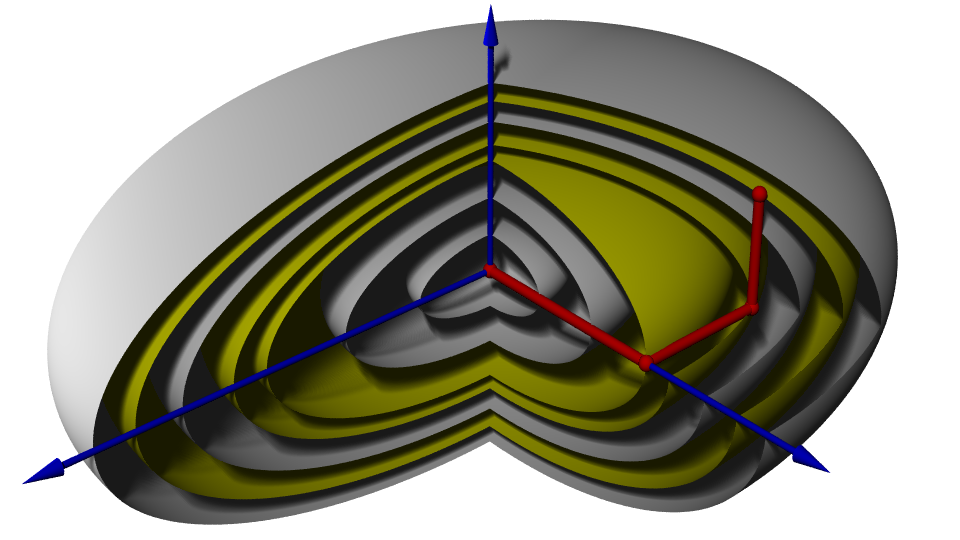
\includegraphics[width=\hsize]{graphics/descent3d.jpg}
\caption{Abstieg entlang der Koordinatenrichtungen f"ur eine Diagonalmatrix
$A$
\label{descent3d}}
\end{figure}
\begin{figure}
\begin{center}
\includegraphics[width=0.45\hsize]{graphics/descent-2.pdf}
\end{center}
\caption{Abstieg entlang der Koordinatenachsen f"ur $A=E$:
die Approximationsfolge konvergiert in nur zwei Schritten zur exakten
L"osung.
\label{descent:exact}}
\end{figure}
F"ur dieses Beispiel wollen wir von einer Diagonalmatrix
$A=\operatorname{diag}(a_1,\dots,a_n)$ und $b=0$ ausgehen.
Wie kann man mit der Abstiegsmethode von einem beliebigen Punkt $x$
zum Nullpunkt absteigen?
W"ahlen wir $e_i$ eine der Koordinaten-Achsen, dann liefert die
Abstiegsformel
\[
x_2=x_1-\frac{e_i^tAx_1}{e_i^tAe_i}e_i
=x_1-x_{1,i}e_i,
\]
d.~h. $x_2$ ist der gleiche Vektor wie $x_1$, ausser in der Koordinate $i$,
die auf $0$ gesetzt worden ist.
W"ahlt man also nacheinander $e_{i_1}$, $e_{i_2},\dots$, dann werden
nacheinander die Koordinaten $i_i$, $i_2,\dots$ zu Null gemacht.
Durch geeignete Wahl der Folge $i_1,i_2,\dots$ zum Beispiel so,
dass die Komponenten $x_{i_1},x_{i_2},\dots$ die absteigend sortierten
Komponenten von $x$ sind, erhalten wir eine Folge Vektoren, die schnelle
gegen $0$ konvergiert, und in genau $n$ Schritten den Nullpunkt exakt
erreicht (Abbildung~\ref{descent3d}).

F"ur $A=E$ h"atte sogar
statt der Koordinatenrichtungen h"atte jede andere Orthogonalbasis
von Vektoren $v_i$ verwendet werden k"onnen. Die Abstiegsformel
\[
x_{i+1}=x_i-\frac{v_i^tx_i}{v_i^tv_i}v_i
\]
produziert dann eine Folge $x_i$ von Vektoren, deren Projektionen auf die
Richtungen $v_i$ abnehmen (\ref{descent:exact}).

Aus diesen beiden Beispielen k"onnen wir ablesen, dass der Abstieg in
maximal $n$-Schritten mit achsparallelen Abstiegsrichtungen
m"oglich w"are, wenn die Niveaufl"achen der Funktion $J(x)$ bereits
achsparallele Ellipsoide w"aren.

Nat"urlich k"onnte man eine Koordinaten-Transformation durchf"uhren,
mit der man die symmetrische Matrix $A$ zu einer Diagonalmatrix oder
sogar zu einer Einheitsmatrix machen kann.
Die Eigenvektoren sind dann die geeigneten Achsrichtungen, entlang derer
der Abstieg erfolgen kann.
Um eine solche Koordinatentransformation zu finden muss allerdings das
Eigenwertproblem f"ur die Matrix $A$ gel"ost werden, was unter anderem
die L"osung der Gleichung $(A-\lambda E)x=0$ beinhaltet. Um mit der
Abstiegsmethode das Gleichungssystem zu l"osen, m"ussten wir also zuerst
das Gleichungssystem l"osen\dots

Selbst wenn die Diagonalisierung ganz einfach w"are, w"are man immer noch nicht
sicher, dass man die bestm"oglichen Abstiegsrichtungen gew"ahlt hat.
Die Idee beim steilsten Abstieg war ja, dass der Gradient die optimale
Richtung ist. Man sollte also einen Abstiegspfad w"ahlen, der mit
dem Gradienten beginnt, dann aber immer nur Richtungen ``senkrecht'' dazu
w"ahlt. Mit so einem Pfad m"usste man in $n$ Schritten die exakte L"osung
finden k"onnen.

\subsubsection{Der Fall $n=2$}
Wir versuchen das eben skizzierte Programm im Falle $n=2$ an unserem
altbekannten Beispiel
\begin{align*}
A&=\begin{pmatrix}1&\frac12\\\frac12&1\end{pmatrix},&
b&=\begin{pmatrix}1\\-1\end{pmatrix},&
x_1&=\begin{pmatrix}2\\0\end{pmatrix}
\end{align*}
durchzuf"uhren. Der Gradient im Punkt $x_1$ ist
\[
v_1=\operatorname{grad}J(x_1)=Ax_1-b=\begin{pmatrix}1\\2\end{pmatrix}
\]
Die erste Abstiegsrichtung ist $v_1$ und die Abstiegsformel liefert
\[
x_2
=
x_1-\frac{v_1^t(Ax_1-b)}{v_1^tAv_1}v_1
=
x_1-\frac{v_1^tv_1}{v_1^tAv_1}v_1
=x_1-\frac{5}{\begin{pmatrix}1\\2\end{pmatrix}^t\begin{pmatrix}2\\\frac52\end{pmatrix}}\begin{pmatrix}1\\2\end{pmatrix}
=\begin{pmatrix}2\\0 \end{pmatrix}
-\frac57\begin{pmatrix}1\\2\end{pmatrix}
=\frac17\begin{pmatrix}9\\-10\end{pmatrix}.
\]
Wenn das angek"undigte Programm funktionieren soll, dann muss der n"achste
Abstiegsschritt bereits die L"osung liefern (Abbildung~\ref{descent3}).
\begin{figure}
\begin{center}
\includegraphics[width=0.55\hsize]{graphics/descent-3.pdf}
\end{center}
\caption{Optimaler Abstieg in zwei Dimensionen, mit Gradient von $J(x_1)$
als erster Abstiegsrichtung.
\label{descent3}}
\end{figure}
Die zweite Abstiegsrichtung ist also
\[
v_2=
x_3-x_2
=\begin{pmatrix}2\\-2\end{pmatrix}-
\frac17\begin{pmatrix}9\\-10\end{pmatrix}
=
\frac17\begin{pmatrix}5\\-4\end{pmatrix}
\]
Die Richtungen $v_1$ und $v_2$ sind offensichtlich nicht orthogonal,
wie der Fall $A=E$ suggeriert hat (Abbildung~\ref{descent:exact}).
Aber es gilt
\begin{align}
v_1^tAv_2
&=
\frac17\begin{pmatrix}5\\-4\end{pmatrix}
\begin{pmatrix}
1&\frac12\\
\frac12&1
\end{pmatrix}
\begin{pmatrix}1\\2\end{pmatrix}
=
\frac17\begin{pmatrix}5\\-4\end{pmatrix}
\begin{pmatrix}2\\\frac52\end{pmatrix}
=\frac17\biggl(5\cdot 2-4\cdot\frac52\biggr)=0.
\label{descent:ortho}
\end{align}
Man nennt zwei Richtungen $v_1$ und $v_2$ mit dieser Eigenschaft
konjugierte Richtungen zur Matrix $A$.

\subsubsection{Das Skalarprodukt zu $A$}
Der allgemeine Fall ist nur deshalb schwierig, weil wir Ellipsen
erhalten, wenn wir die Niveau-Linien von $J(x)$ aufzeichen.
Und auch nur, weil wir darauf bestehen, als L"ange eines Vektors den
Wert $v^tv$ zu verwenden.
W"urden wir stattdessen als L"angenmass die ebenfalls positive
Gr"osse $v^tAv$ verwenden, dann w"aren alle Punkte mit gleichem $J(x)$
gleich weit von der L"osung entfernt.
Wenn $v^tAv$ das L"angenmass sein soll, dann muss nat"urlich auch das
Skalarprodukt ersetzt werden, statt des gew"ohnlichen Skalarproduktes
$\langle x,y\rangle =x^ty$ muss man also das verallgemeinerte
Skalarprodukt $\langle x, y\rangle_A=x^tAy$ verwenden.

Die zweite Abstiegsrichtung k"onnen wir also wieder den Gradienten
verwenden, aber in Richtung $v_1$ ist ja schon der optimale Abstiegsschritt
durchgef"uhrt worden, wir m"ussen also die Komponenten des Gradienten
in Richtung von $v_1$ abziehen:
\begin{align*}
v_2'&=\operatorname{grad}J(x_2)=Ax_2-b
&\Rightarrow&
&
v_2&=v_2'-\frac{\langle v_1,v_2'\rangle_A}{\langle v_1,v_1\rangle_A}v_1.
\end{align*}

\begin{beispiel}
Im altbekannten Beispiel bekommen wir
\begin{align*}
v_2'&
=Ax_2-b
=\begin{pmatrix}1&\frac12\\\frac12&1\end{pmatrix}\frac17\begin{pmatrix}9\\-10\end{pmatrix}-\begin{pmatrix}1\\-1\end{pmatrix}
=\frac17\begin{pmatrix}4\\-\frac{11}2\end{pmatrix}
 -\begin{pmatrix}1\\-1\end{pmatrix}
=\frac17\begin{pmatrix}-3\\\frac32\end{pmatrix}
\end{align*}
Dies ist aber nicht die Abstiegsrichtung, davon muss erst die Komponente
in $v_1$-Richtung entfernt werden. Dazu m"ussen die Skalarprodukte
$\langle v_1,v_1\rangle_A$ und $\langle v_1,v_2'\rangle_A$ berechnet
werden
\begin{align*}
\langle v_1,v_1\rangle_A
&=
v_1^tAv_1
=
\begin{pmatrix}1\\2\end{pmatrix}^t
\begin{pmatrix}1&\frac12\\\frac12&1\end{pmatrix}
\begin{pmatrix}1\\2\end{pmatrix}
=
\begin{pmatrix}1\\2\end{pmatrix}^t
\begin{pmatrix}2\\\frac52\end{pmatrix}=7
\\
\langle v_1,v_2'\rangle_A
&=
v_2'^tAv_1=
\frac17
\begin{pmatrix}-3\\\frac32\end{pmatrix}^t
\begin{pmatrix}2\\\frac52\end{pmatrix}
=\frac17\biggl(-6+\frac{15}{4}\biggr)
=-\frac9{28}
\\
v_2&=
v_2'-\frac{\langle v_1,v_2'\rangle_A}{\langle v_1,v_1\rangle_A}v_1
=
\frac17\biggl(
\begin{pmatrix}-3\\\frac32\end{pmatrix}
+\frac9{28}
\begin{pmatrix}1\\2\end{pmatrix}
\biggr)
=
\frac{15}{196}\begin{pmatrix}-5\\4\end{pmatrix}.
\end{align*}
Der Vektor $v_2'$ hat genau die Richtung, die wir als die optimale
Richtung im vorangegangenen Beispiel erkannt haben.
\end{beispiel}

\subsubsection{Optimale Abstiegsrichtungsfolge}
Das Skalarprodukt $\langle\cdot,\cdot\rangle_A$ kann also dazu verwendet
werden, aus der Folge der Gradienten $v_i'=\operatorname{grad}J(x_i)$
durch Orthogonalisieren eine Folge von Abstiegsrichtungen zu 
konstruieren.
Das Orthogonalsierungsverfahren nach Gram-Schmidt liefert die
orthogonalisierten Vektoren
\[
v_i=v_i' - \sum_{j=1}^{i-1}\frac{\langle v_i,v_j\rangle_A}{\langle v_j,v_j\rangle_A}v_j
\]
Diese Formel kann sogar noch etwas vereinfacht werden, wenn man die
Vektoren $v_j$ normiert bez"uglich der L"angenmessung mit dem Skalarprodukt
$\langle\cdot,\cdot\rangle_A$.
Die L"ange eines Vektors in diesem Skalarprodukt ist
\[
|v|_A=\sqrt{\langle v,v\rangle_A}.
\]
Wir definieren die Folge der Vektoren $v_i$ daher wie folgt:
\begin{align}
v_{i+1}'&=\operatorname{grad}J(x_i)=Ax_i-b
\notag\\
v_{i+1}''&=v_{i+1}'-\sum_{j=1}^{i}\langle v_j,v_{i+1}'\rangle_A v_j
\label{cg:ortho}
\\
v_{i+1}&=\frac1{|v_{i+1}''|_A}v_{i+1}''
\notag
\end{align}
Mit dieser Richtung f"uhrt man dann den Abstiegsschritt durch.

Damit haben wir jetzt ein Iterationsverfahren konstruiert, welches nicht
nur immer bessere Werte liefert, sondern in $n$ Schritten sogar die exakte
L"osung.
Es hat aber immer noch einige Nachteile. Einerseits m"ussen alle bisherigen
Abstiegsrichtungen gespeichert werden, und die Formel (\ref{cg:ortho}) wird
mit jedem neu berechneten Vektor $v_j$ umfangreicher auszuwerten.
Die sp"ateren Schritte des Verfahrens sind also langsamer.
Das es auch bei der Konvergenzgeschwindigkeit noch Verbesserungspotential
gibt, zeigen die folgenden Beispiele.

\begin{beispiel}
Man l"ose des Gleichungssystem mit 
\begin{align*}
A&=\begin{pmatrix}
     1&\alpha&     0&      &      \\
\alpha&     1&\alpha&      &      \\
     0&\alpha&     1&\smash{\ddots}&      \\
      &      &\ddots&\ddots&      \\
      &      &      &      &     1
\end{pmatrix}
&
b&=\begin{pmatrix}1\\1\\1\\\vdots\\1\end{pmatrix},
&
x_1&=\begin{pmatrix}1\\0\\0\\\vdots\\0\end{pmatrix}.
\end{align*}
Mit dem CG-Verfahren, und bestimme die Konvergenzgeschwindigkeit.

\begin{figure}
\begin{center}
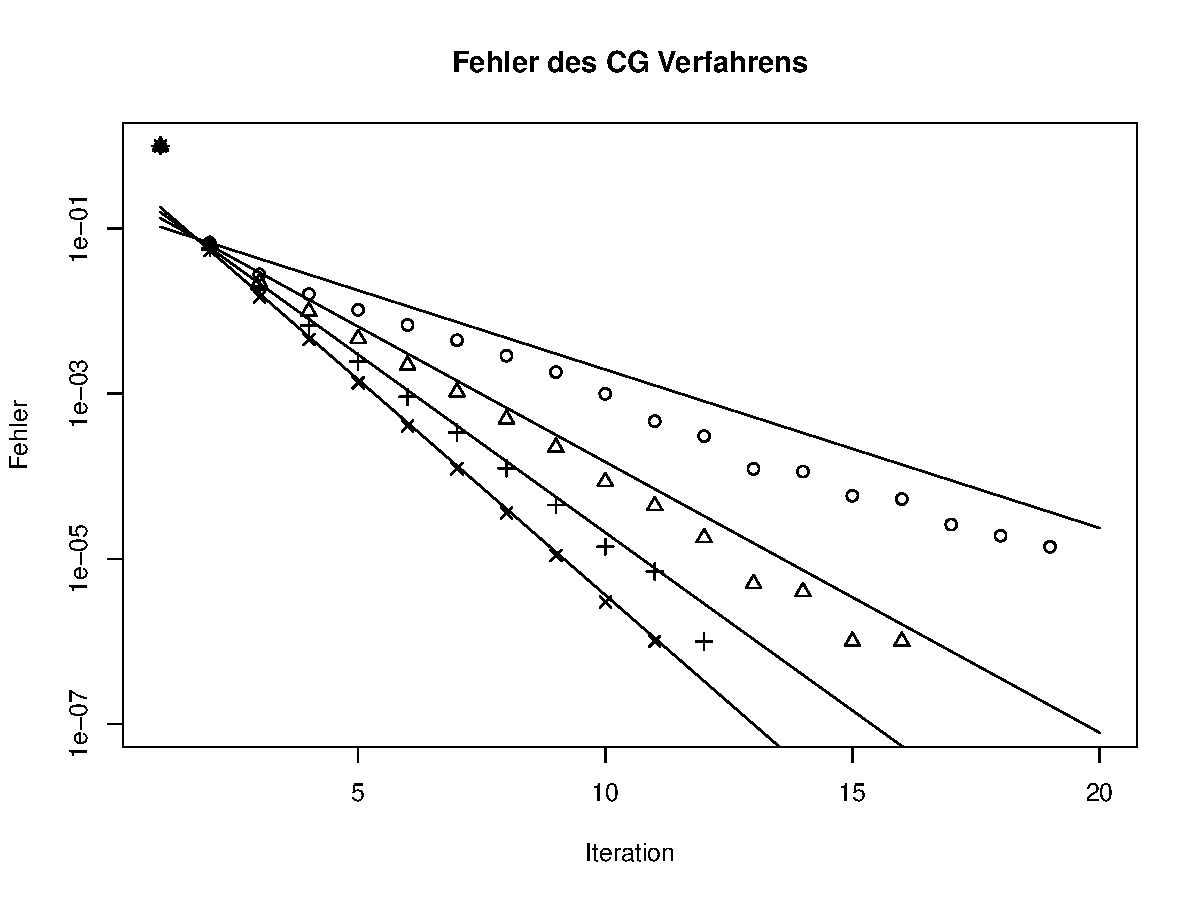
\includegraphics[width=\hsize]{graphics/cgresults.pdf}
\end{center}
\caption{Fehler des CG-Verfahrens in Abh"angigkeit von der Anzahl
Iterationsschritte f"ur verschiedene Werte von $\alpha$.
Zum Vergleich jeweils die Gerade mit Steigung
$q=(\sqrt{\kappa_2(A)}-1)/(\sqrt{\kappa_2(A)}+1)$.
\label{cg:example}}
\end{figure}
Die Abbildung \ref{cg:example} zeigt die Restfehler f"ur $n=20$
in Abh"angigkeit von der Anzahl Iterationsschritte.
Es ist klar, dass nach 20 Schritten die exakte L"osung gefunden wird, also
kein Fehler mehr "ubrig bleibt.
Wie zu erwarten nehmen die Fehler ungef"ahr in geometrischer Folge ab,
doch nur f"ur vergleichsweise kleine Werte von $\alpha$ ist die Konvergenz
einigermassen schnell.
F"ur $\alpha = 0.5$ hat das Resultat auch nach 19 Schritten nur vier
korrekte signifikante Stellen.
\end{beispiel}

Der CG-Algorithmus garantiert zwar, dass die exakte L"osung gefunden
wird, aber er ist nicht notwendigerweise viel schneller als die bisher
gefundenen Algorithmen.
Im Folgenden muss auch daf"ur die Ursache gefunden werden, und es m"ussen
Methoden entwickelt werden, mit denen die schnelle Konverenz sichergestellt
werden kann.

\subsubsection{Orthogonalit"at der Fehler}

\subsubsection{Pr"akonditionierung}

